%http://cs.pugetsound.edu/~jross/courses/cs240/project/requirements/
%Animation Group
\documentclass[12pt]{article}
\usepackage{titlesec}
\usepackage{graphicx}
\usepackage[labelformat=empty]{caption}
\titleformat{\section}[block]{\bfseries}{\thesection.}{1em}{} 
\titleformat{\subsection}[block]{\hspace{2em}}{\thesubsection}{1em}{}
\titleformat{\subsubsection}[block]{\hspace{2em}}{\subsubsection}{1em}{}
\titleformat{\paragraph}[block]{\hspace{5em}}{\paragraph}{6em}{}
\def\changemargin#1#2{\list{}{\rightmargin#2\leftmargin#1}\item[]}
\let\endchangemargin=\endlist 
%\setlength{\parindent}{4cm} % Default is 15pt.

\begin{document}

% Front Page
\begin{titlepage}
	\begin{center}
	\huge  Edith \\
	\vspace*{\fill}%
 	\huge \textbf{Animation System \\Final Report}
	\bigskip 
	\rule{130mm}{.1pt}
	\textsc{\textbf{December 20, 2013} \\ }
	\vspace*{\fill}%
	Eric Lund \\
	Kramer Canfield \\ 
	Zeke Rosenberg \\
	Calder Whiteley \\
	Jon Youmans
	\end{center}
\end{titlepage}

\section{\emph{\Large Project Summary}}%Create a section for the introduction
\subsection{Edith System}
\begin{changemargin}{1cm}{0cm} 
Edith is a 2D, web-based system to help young students learn to program and get excited about computer science. The system allows students to program relationships among objects in a virtual world, in order to create animations. It offers several useful capabilities: users are able to create objects for their story using a graphical, drag and drop interface; specify animated behaviors for these objects using a visual programming language; and view their completed animations.

\end{changemargin} 
\subsection{Animation System}
\begin{changemargin}{1cm}{0cm} 
The Animation System module is important because it includes the core animation frameworks and specifications of how the animations are produced. In a visually-based programming environment, this module is clearly important because it provides animations without requiring the user to have any knowledge of a scripting language or computer graphics concepts. The Animation Module accepts a properly formatted instruction list as a String of generated JavaScript code to evaluate and construct a series of animations which show up on the canvas. The canvas is installed in the final UI within the webpage by the Story Creator Module. To help with the construction of the list of instructions, we provide the Visual Editor developers with a formal API specification to give details on exactly what our module is expecting and how to call our animation methods.
\end{changemargin} 

\section{\emph{\Large Development Procedures}}
%\begin{changemargin}{1cm}{0cm} 
Our early development mostly consisted of group brainstorming and planning.  Our development process originally seemed to follow the plan-based process but we quickly morphed to the agile system.
We started our development with getting the basic animation and canvas functions implemented.  Once that was implemented we quickly moved on to JSON input parsing.  In parallel with the JSON parsing implementation we developed an Animation API which documented the animation blocks and their parameters.  As we added more advanced animations and refined our JSON format we updated the API to reflect these changes.  The final step to our implementation was creating the ``hook" that allowed the timeline to play the animation sequence.  Debugging was an ongoing aspect of the entire development process.
We tested our systems by creating animation instruction sets which utilized our animation blocks in as many was as we could think of.  
All five of us took part in the software development, oftentimes led by Eric as he had the best grasp on the functionality of the oCanvas Library that we utilized.  Kramer handled the group liaison duties and Calder built the initial API structure.  Updating and maintaining the API content was handled as needed by all of the group members.
Development and implementation went incredibly smoothly for our group and when we hit stumbling points we worked efficiently as a team to quickly overcome them.
%\end{changemargin}


\section{\emph{\Large Requirements Evaluation}}
%\begin{changemargin}{1cm}{0cm} 
In the beginning of the project, our set of requirements and overall system functionality had a wide degree of specificity. Fortunately, we were able to have our code and module structure be adaptable. Our module design and system structure did change dramatically throughout the engineering process, but we were still able to accomplish most of our main use-case and requirements.\\

\large Non-functional Requirements\\\\
We mostly accomplished both non-functional requirements of providing documentation and instructions on which animations we could provide and how our module interacts with the rest of Edith. We accomplished this by creating a formal API of animation methods built-in to our JavaScript file.

\textit{``Ease-of-Use: Specific documentation of options for animation provided to the ”Drawer” on animations that we can provide."(Requirements Specification)}\\
This non-functional requirement deals with usability and was incredibly helpful in the software-engineering process. The API that we created was helpful in creating the ties between the visual editor’s module and our provided code.
\textit{``Documentation: Specific documentation of instructions provided to the ”Taker” on how to receive the dynamic picture frame (the canvas).(Requirements Specification)"}\\
This non-functional requirement was only partially met. We did not end up using a dynamic picture frame, but we did give instructions to the Story Creator team, who managed the final webpage user interface, of how to add the special oCanvas library and canvas that we needed for our animations to display properly.\\


\large Functional Requirements\\\\
\textit{The Animation System would accept JSON instructions to be defined in an API that gave instructions for types of animations, durations and other parameters.}\\
This requirement had many changes. There was some misunderstanding about how the final system would work for a long time at the beginning of implementation. This requirement was written when our perception was that we would have our own canvas and possibly an HTML file with which to write in buttons and such for playback controls, etc. In the final Edith implementation, the animation canvas is just a canvas plopped onto the main page as a piece of the website. Thus, the actual HTML of the page was handled by the Story Creator team, and Animation provided our code solely via an external JavaScript file. There was then a second period of misunderstanding in which the requirements changed, and we were under the impression that this external JavaScript file would be called on by the Visual Editor team so their functions would call our code's functions. Again, requirements changed; in the final implementation of Edith, we went with an altogether different solution. Our final solution contains a `animationMain()' method, which simply runs the JavaScript eval() function on a String of JavaScript code. This way, the Visual Editor team was able to construct the string using their blocks. These blocks simply added text to the string that was the aforementioned hooks to our program. The play button from the Story Creator team then simply called our main() method, with the parameter of the Visual Editors string of JavaScript code, which we automatically evaluate and run. If there are any errors in the string, it will crash just as normal JavaScript would. This is intended as we want to simulate a real programming experience and not something that worked every time. \\

\textit{The JSON instructions would be read by the animation system, which would then create animations and sounds in a frame based system.}\\
As mentioned above, we made the choice to use the oCanvas external library to ease the production of an object oriented experience for the user in the end. In the end, the use of the oCanvas turned out to be both a blessing and a curse. It definitely simplified things for us in the beginning, but as we looked towards some of our other requirements or even just tried to do additional things with our animations we were hampered by the system. The oCanvas uses animation queues for sprites to move around the queue. In regards to the sprites, we met our requirements, as that is how we described the animations to work. Initially,we had the notion that our animations would work by producing a series of frames, which we could easily store in an array, then rapidly display on the screen in series. This did not end up working, because the oCanvas does animations as a queue of actions with a length. If you want to do certain series of animations, it would actually be easier in a custom system. For example, if you want a sprite to begin moving across the screen then midway through the motion begin spinning as well, you run into a few issues. Calling move and then rotate will result in the sprite moving to the location, stopping, and then rotating. To get the desired animation you would need to start a new queue, and put the rotation in there. This still doesn’t solve the issue, because now your sprite would start moving and spinning at the same time. So you would really have to make a new queue, put a wait() call in one queue, and then add the rotate method to the new queue. This appraoch still does not solve the issue, because now your sprite would start moving and spinning at the same time. So the solution is to make a new queue, put a wait() call in one, and then add the rotate to that. In our initial understanding, we thought that our methods would have some sort of a duration parameter as well as a timestamp parameter that told the system when it needed to be called. Because of the odd nature of the queue within the oCanvas, once we were overly reliant on that (which unfortunately came in the beginning of our development) it was very difficult to find work-arounds without sacrificing all of our previous work and starting over.\\

\textit{The Animation System provides video output to be taken by another group and drawn onto the canvas, simultaneously playing associated sound files in a standard audio format.}\\

This requirement was half met. We did draw our animations onto a canvas that another group gave us a reference to, but it is not just a video file. Our animations work through an interactive display painted on a regular HTML 5 canvas, which uses the oCanvas library. The downside of this is that there is not currently a way to export a video file created using Edith. However, the framework is there for videos and projects to be fairly easily loaded by another user into Edith, although that functionality isn’t implemented. There was a period of time when we considered adding audio to our videos, and our earlier integration demos actually featured a working video and audio combination, as well as an interface for easily associating sound files with a particular animation. However, there was no other group working on any of the other means that were needed for the audio to work, and they were all overwhelmed with their development. What would have been needed is a way to share/access audio files via sharing framework, a way to upload your own sound file or access a stock database of files, and an interface for scrolling through given sounds and attaching them to animations, which in all would have required Sharing Framework, Object Creator, and Visual Editor to all do additional work which was not specified in the requirements. This is a good example of how we did not completely think through how we wanted the sound to work with the rest of the project. Our early requirements did not make it clear what would need to happen with other groups in order to include sounds, so it was lost in favor of other features. \\

\textit{The Animation System will have playback control functionality that will allow a user to pick a time to begin their video from, and watch it from their to enable easier testing and editing of videos within Edith}\\

This requirement was not met. As described above, we ran into problems with the way that we chose to implement the object-oriented nature of our sprite animations, specifically in oCanvas. Because we began implementation using the oCanvas without thinking through our processes, it was very difficult to backtrack and find a solution for playback controls. We could have implemented a very inelegant rudimentary system that enabled the user to jump to specific instructions that they had chosen, or even to a specific time, but the outcome would have been quite messy. Problems that we anticipated were instructions that would effectively be `lost’ if a user attempted to jump to a time that was between the start and end of an animation. This implementation would have been moderately useful for a user who wanted to jump to the end of a very long video, but we felt that it would have been buggy with no ways to fix the issues. Again, this was a product not only of our reliance on the oCanvas but also of a failure to comprehend how we would implement our requirements. In short, our requirements were initially too vague. In the end, we did not even implement a simple start/stop function. This is because the oCanvas has no way of stopping and resuming an animation.
%\end{changemargin} 



%\end{changemargin}

\section{\emph{\Large System Design} \Large \& \emph{\Large Architecture}}
Animation teams final implementation is contained within one javascript file and contains a list of functions that can be utilized by other groups. These functions are primarily functions that animate objects (sprites) on the canvas but also include a few functions that allows for the ability to add sprites onto the canvas. To achieve this, our design utilizes and relies heavily on an external library called oCanvas. oCanvas is a JavaScript library that is intended to make development with a HTML5 Canvas easier. Instead of working with pixels, oCanvas allows for an object oriented interface allowing animations to be applied to objects, in our case, sprites. oCanvas can be thought of as strapping extra functionality onto a preexisting HTML5 canvas as all of the generic HTML5 canvas functions are still available and can be interweaved with any of the oCanvas functions. More information and documentation about oCanvas can be be found at their website: http://ocanvas.org. Because our code contained in one JavaScript file, we have appended the oCanvas library directly into our code as it can not be imported in line as it could be with HTML. \\

In order to begin using the animation functions the user needs to create a HTML5 canvas and assign it an ID. This ID can then be fed into our function called wrapHTMLCanvasToOcanvas(HTML5canvasID, background) which takes the HTML5 ID and a background color. This function simply takes the HTML5 canvas ID and calls the oCanvas function create() which creates the oCanvas. Our method then returns that oCanvas object. As stated above, this methods basically extends the HTML5 canvas adding more functionality to it -- it does not actually create a new canvas. After attaining the oCanvas object, sprites can then be added by calling the function addSprite(theOCanvas, image, width, height, xcoord, ycoord). The first parameter to this method is the oCanvas object which is returned from the first function wrapHTMLCanvasToOcanvas. The image parameter is a string of an image path to the image to be represented as the sprite. The remaining parameters deal with the size and location of the sprite. Once those steps have been completed, the user can animate the sprite using any of our animation functions. \\

This process can be simplified to a series of 4 steps:
\begin{itemize}
\item Create HTML5 canvas assigning it an ID.
\item wrapHTMLCanvasToOcanvas() to attain an oCanvas object.
\item Add sprites by calling addSprite().
\item Animate the sprites with the provided animation functions.\\
\end{itemize}

Below is a System state diagram that shows a sample implementation.

\begin{figure}
\caption{Figure 1. System State Diagram}
  \centering
    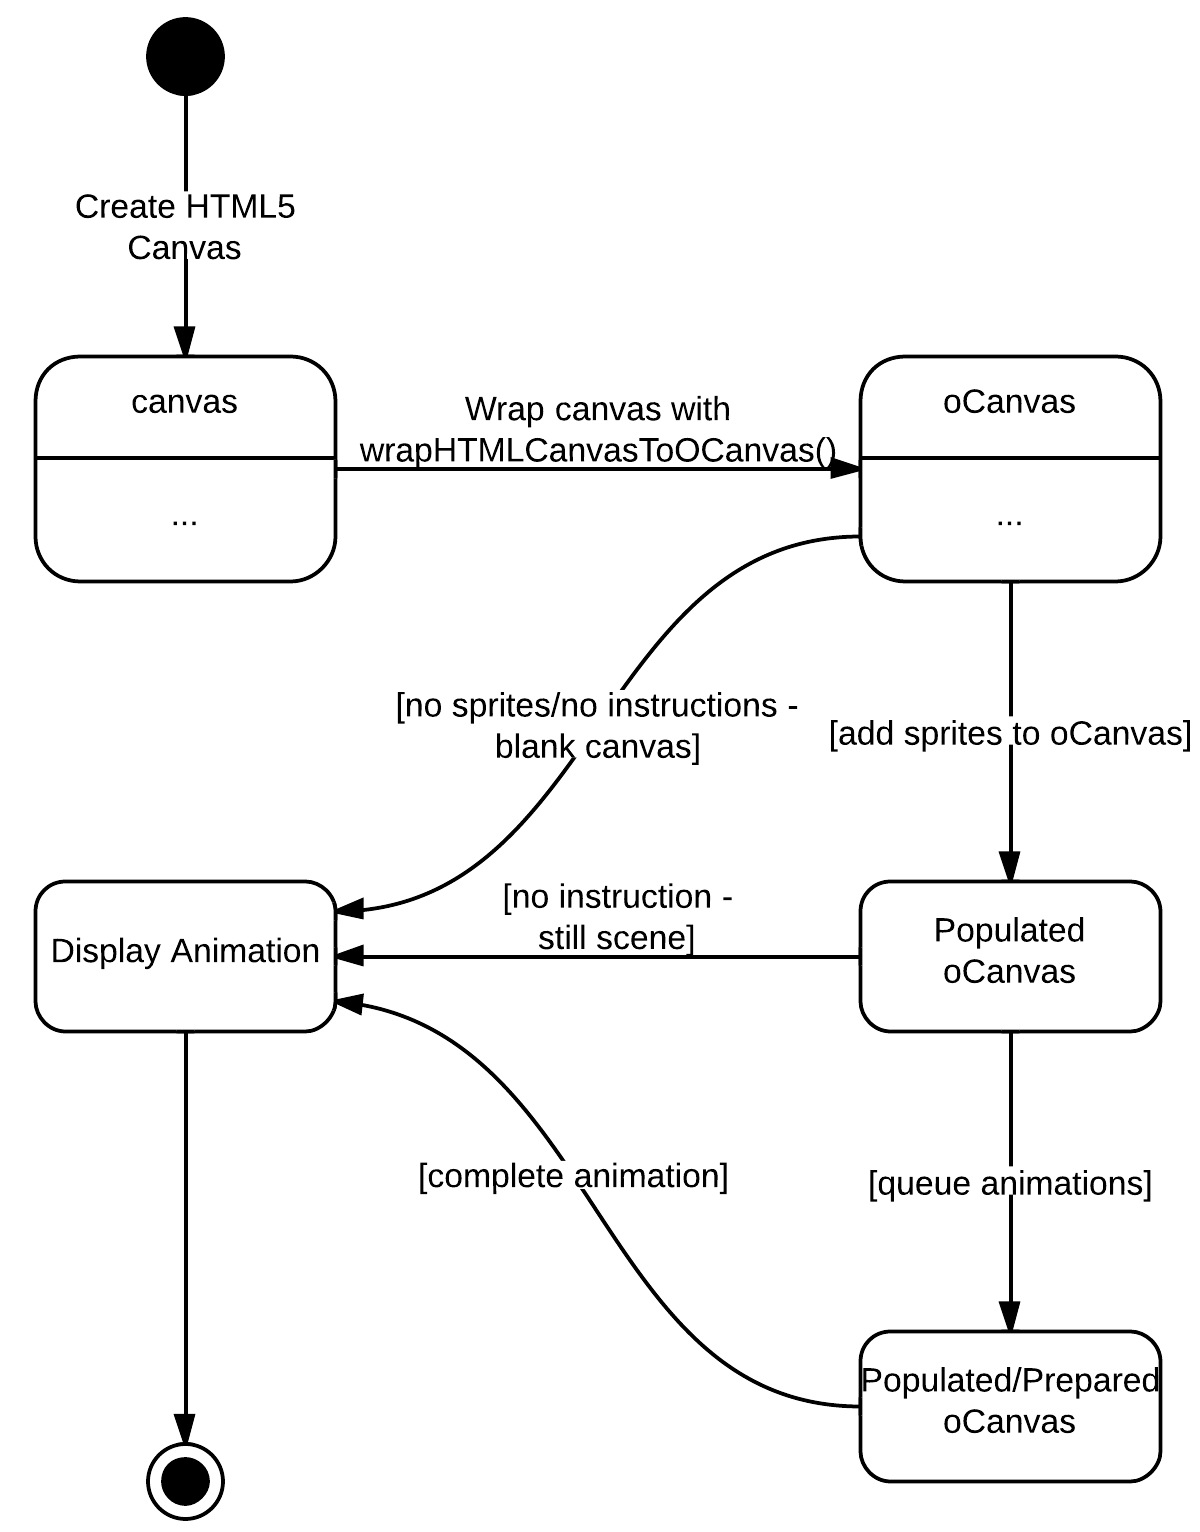
\includegraphics[scale=.3]{animation-statediagram.png}
    \caption*{After creating an HTML5 canvas user calls the wrapHTMLCanvasToOCanvas() to create oCanvas object. At this point sprites and instructions can be added to be displayed on the canvas object.}
\end{figure}
    

 \newpage
Our animation functions include a generic animate function and a series of pre-defined animations created by our group. The generic function is called move() and can animate a sprite in any combination of the x-axis, y-axis, and z-axis (rotation). This function is intended to be used for simple animations but also allows the flexibility for the programmer to call a series of move functions to create a more complex animation. Our pre-defined animations include jump, double jump, move left, move right, move up, and move down which can be called in addition to the generic move. The main content behind all of the animation functions is a animation block provided by the oCanvas library. This animation block allows for many optional parameters that can be used to produce different effects. Some of the effects that we utilized are easing functions, duration time, and animation queues. \\ 
\paragraph{}
The animation system is conveniently documented in a clean browsable API. Each method is described in brief detail within the API site with all parameters listed and defined below. This documentation is intended for other developers who are using the animation system and provides all the details necessary to call and handle animation methods.
\\
\begin{figure}
\caption{Figure 2. Animation System API}
  \centering
    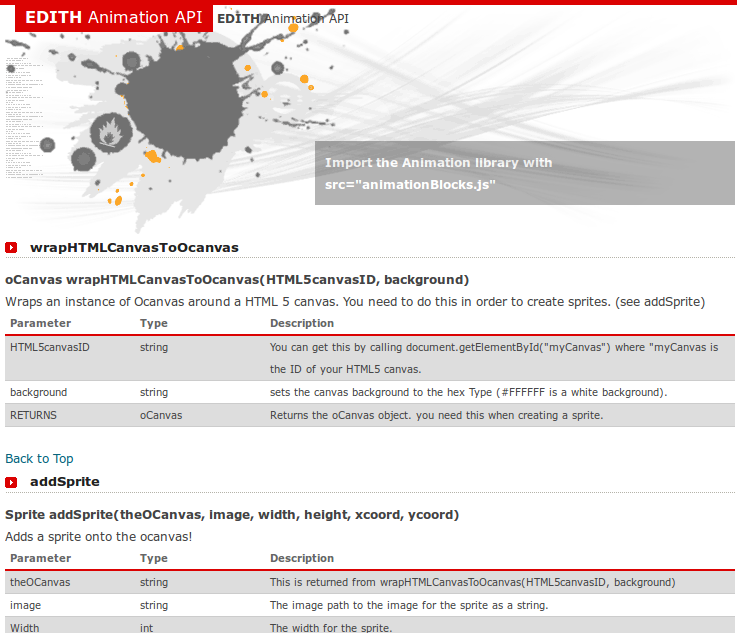
\includegraphics[scale=.55]{api-screenshot.png}
    \caption*{All animation methods are documented in an accessible API.}
\end{figure}

\newpage
\section{\emph{\Large Individual Reflections}}
\subsection{Eric Lund}
\begin{changemargin}{1cm}{0cm} 
          Many challenges came up through development both technical and organizational throughout the whole development process. One of the biggest problems that stood out the most to me and falls in both the technical and organizational aspects was using GitHub for our source control.  The idea behind Git is awesome, and should make the development process much easier and efficient when working with a group of people but I felt that in our case it held us back. It was a technical problem in that none of the members in our group had really worked with Git, or even a true source source control system prior to this project. There were multiple times in the beginning of development in which we actually lost some work (nothing substantial, luckily) due to us not knowing the technical aspects of how Git/GitHub worked. Though the development process we gained a lot of experience with works Git and I think it ended up being a helpful tool — especially when we got to the integration periods with the other groups. The organizational challenge working with Git came by us not sufficiently managing our files in our branch. I was very hesitant (and I think I can speak for the team as well) in changing directories for files and moving folders around as it was only followed up by a series of merge conflicts and tracking problems. Because of that, our branch got messy real fast and wasn't as organized as it should of been. As a group it wasn't that big of a deal but if other groups wanted to look at what we had it would of been hard for them to find what they were looking for. \\
          
           Our group utilized many software engineering techniques during the development process but what stood out to me the most was our communication abilities. Our group had several meetings in which all of our members were able to attend and stay up to speed with the current development process. We even had several meetings that we didn't do any coding but rather talked about how we were going about on our implantation and what our next steps were going to be. Reflecting back this really made the whole process much easier.\\
           
           If I were to redo the whole process there are two things I would definitely do. One of which would be to get a better grasp of Git/GitHub. I feel it would be beneficial if the whole group took time away from development to make sure we all knew and felt comfortable working with Git and also discuss as a group, how we would use it. Another thing I would do is communicate more with the other groups that directly affect what we are developing. As I said earlier, I felt the communication was exceptional in our group but it would of been even better if we extended that out to the other groups as well by staying updated on their current status and implementation. I had a great experience with my group members and felt like we accomplished the task at hand. 
\end{changemargin} 
\subsection{Kramer Canfield}
\begin{changemargin}{1cm}{0cm} 
There were more than a few challenges in doing this project. For technical challenges, we had to learn Git and GitHub, one of the first real programs that I have had to learn to use mostly on the command-line. Most of the time, using Git was helpful, but incredibly troublesome and most of the time that we had errors, we would delete the local copy and just reclone from our branch on GitHub. Unfortunately, I feel like we didn't take time to learn it in as much detail as we should have and therefore, we could not take advantage of it's power. Another technical hurdle was learning JavaScript, which I had never written before. It was more difficult to learn that I thought; even though I am more practiced now, I still do not quite feel comfortable with it. One organizational challenge was getting the entire group together for meetings. We did okay as it turns out, but it would have been nice if we had more meetings with the whole group. That being said, the group meetings that we did have were extremely valuable for brain-storming ideas and discussing goals for the project. We overcame scheduling issues by making a Google Calendar that was shared between us as well as sending text messages to remind each other about meeting times. To avoid confusion, we almost always met in the same place.\\
Software engineering techniques we used include good intra-group communication such as making sure we were all caught up on recent events that affected our work. I also feel like we relied on each of our own strengths in order to meet important deadlines because the focus seemed to be on the deliverables. The work was more or less evenly split up, but we each mostly worked on tasks that required our strengths rather than taking time to learn a skill more in depth. For example, I worked on documentation more than JavaScript programming, but I still pulled my own weight.\\
If I were to restart this project, I would want to have more entire-class meetings so we can all discuss the project and what the end goal ultimately is. I feel that there was a lot of ambiguity in what the final product would actually do until we got most of the way through the semester. I would also want to practice more with Git/GitHub, and JavaScript as those were the most difficult to learn.

\end{changemargin} 
\subsection{Zeke Rosenberg}
\begin{changemargin}{1cm}{0cm} 
The Animation team’s biggest struggles were in the definition of what we needed to accomplish. I don’t think any of us had a very firm grasp on Edith as a whole project at the beginning, and our requirements reflected that—they were vague and ill defined. This caused us a lot of problems because we continuously got ahead of ourselves without planning out what we needed to do. This worked fine for us as an isolated team, because the five of us was a small enough team and we were all flexible that we could practice a sort of agile development in which we would change course depending on what needed to be done. However, this did not work very well within the scope of the larger scale Edith project, as there were lots of miscommunications with other groups about what we were providing and how it would work. 
	I think that most of our problems could have been solved by just a little more planning before we actually began working on anything, as well as thinking about the ramifications of our design decisions as we were making them. One of the places where we got ahead of ourselves the most was with the oCanvas, because it hampered our development on several other key deliverables including exporting videos, a frame based animation system, and playback controls. That being said, we were able to use it to get what we wanted to accomplish done. This is both a technical and an organizational failure which fit together. The Organizational failure was in our lack of preemptive planning and strategy, and our technical problems stemmed from that lack of examining our overall approach to animations. The takeaway from both of these is that we need to in the future spend more time on our requirements, and make them as detailed as possible so we have a very clear roadmap to go by. This was difficult, because we were trying to keep our requirements from being overly technical, but without the technical details we were somewhat lost in where to begin with our development. 
	Our use of Git was very interesting. It was definitely effective for sharing files between us, but not much more than that—I don’t think we took full advantage of the possibilities for testing by branching, so we ended up just making lots of unnecessary additional files to test things with. Additionally, the most productive times that we had occurred when working as a group in the same room, in which git helped us track changes and keep everyone following along on different computers, but in the end we were coding in a style much similar to pair programming and just working together. This was an effective way for us to work because it also enabled us to use real life aides as simple as pencil and paper drawings of what we wanted to happen our diagrams of interactions between components. 
	If I was starting Edith all over again, the first thing that I would do is spend more time in the beginning on the requirements, and make sure that they matched up to all of the other groups. If I was doing the animation system, I would probably prefer to work from scratch (without oCanvas), because while it would be much more daunting in terms of man hours it would also allow us to include a lot more functionality such as the playback controls or more interesting custom animations (like scaling or color changing). 
\end{changemargin} 
\subsection{Calder Whiteley}
\begin{changemargin}{1cm}{0cm} 
Aside from the initial  difficulty defining our team's deliverable goals, I found the largest challenge to be our early trouble with Git and GitHub.
We had several occasions early on where the only way to push content was to delete the entire local repository and re-clone from the 
branch master.  This came about because of some unknown error having to do with pulling from the branch master.  Since you are 
required to be up to date on your local files prior to pushing, the inability to successfully pull updates from our branch master inhibited 
our progress and lost us several iterations of our early work.  Once those issues magically disappeared we had little to no further trouble 
with Git and GitHub for the remainder of the project.
As a group we worked incredibly well together.  When members were unable to make meetings the laid-back, agile-system quality of our 
team dynamic allowed us to effectively fill in for each other as needed, contribute from other locations as well as get quickly caught back up.
Early meetings involved group brainstorming and mapping but rather quickly we moved into a ``show-then-explain" method of conveying ideas 
and getting work done.
Towards the end of the project our group lost purpose as all of our modified deliverable conditions had been met.  Inter-team communications 
were much less mature than our own member-to-member interaction.  As a result offering our services to other groups was relatively unfeasible.
\end{changemargin} 
\subsection{Jon Youmans}
\begin{changemargin}{1cm}{0cm} 

Initially, I found the biggest challenge to be concretely defining the goal of our team. It was difficult to discuss and vet approaches to the problem at hand without being positively clear about the target. As the project continued the goal began to take shape and it became easier to see where the group's effort and focus belonged.

Organizationally, our team had a relaxed group structure that made it easy to contribute when our schedules conflicted. This allowed team members to manage their time effectively and balance their efforts for the project with demands from other classes.

While the group had a sound background in programming, as Eric said above, our version control experience was minimal at best and GitHub caused a lot of frustration for us. Its value is really clear but we continually marched forward focusing on development without stopping to get truly comfortable with what git has to offer. Version control was a very valuable concept to me and possibly the most import thing I took away from this class. I intend to improve my understanding of git as I continue with software development.

LaTex was also a valuable technology to be introduced to. I plan to increase my familiarity with it going forward as well.
    
While our development style began with a large planning session our heading changed significantly throughout the project. This occurred most notably after integration meetings as the big picture became more firmly established. We designed our module to be somewhat flexible to changing requirements but the passive nature of the animation system, in the sense that it provides methods to be called by other systems, kept our team mostly insulated from sudden changes in requirements throughout the semester.
    
If we were to start this project again I would begin with more serious use cases and an immediate intergroup meeting to establish the group roles a little more clearly. Internally, I think we solved the problem quite efficiently by taking advantage of an existing animation library and tailoring it to the project. That being said, I think some of the reasoning behind our design comes from the pressure we had to firm up our implementation before other teams could specify the functionality they required. 

\end{changemargin} 


\section{\emph{\Large Glossary} \Large  \& \emph{\Large References}}

The oCanvas library: www.ocanvas.org
	
\end{document}
